% Mathematical Environments
\newtheorem{theorem}{Theorem}[section]
\newtheorem{lemma}[theorem]{Lemma}
\newtheorem{definition}{Definition}[section]
\newtheorem{assumption}{Assumption}[section]
\newtheorem{proposition}{Proposition}[section]
\newtheorem{corollary}{Corollary}[section]

% Custom Math Commands
\newcommand{\Tr}{\mathrm{Tr}}
\newcommand{\rank}{\mathrm{rank}}
\newcommand{\R}{\mathbb{R}}
\newcommand{\Sym}{\mathbb{S}}
\newcommand{\norm}[1]{\left\lVert#1\right\rVert}
\newcommand{\inner}[2]{\langle #1, #2 \rangle}

\section{Mathematical Foundation}

The advent of massive-scale optimization has exposed the inherent limitations of classical convex algorithms. Semidefinite Programs (SDPs) provide exact convex relaxations for NP-hard combinatorial geometries by optimizing linear objectives over the cone of positive semidefinite matrices. However, enforcing the positive semidefinite constraint utilizing logarithmic barrier functions demands the calculation of a dense Hessian matrix at each iteration, resulting in polynomial time complexities that render large-scale problems intractable due to memory exhaustion.

To circumvent this, the Burer-Monteiro (BM) approach utilizes a non-linear substitution, replacing the continuous variable matrix with low-rank factorization. This drastically reduces dimensionality and implicitly enforces the semidefiniteness constraint. Yet, this introduces a highly non-convex objective landscape characterized by equivalence classes, quotient manifolds, and saddle points. 

This section introduces the mathematical and optimization perspectives required to understand why gradient-based local search algorithms succeed on these non-convex manifolds, anchored entirely by the geometric guarantees of the Barvinok-Pataki bound.

\subsection{Positive Semidefinite (PSD) Matrices}
A symmetric matrix $Y \in \Sym^n$ is Positive Semidefinite (denoted $Y \succeq 0$) if, for any non-zero vector $v \in \R^n$, the quadratic form evaluates to a non-negative scalar:
\begin{equation}
v^T Y v \ge 0
\end{equation}
Geometrically, a PSD matrix ensures that the applied linear transformation never reflects a vector into its exact opposite half-space, guaranteeing all eigenvalues are non-negative.

\subsection{Semidefinite Programs (SDPs)}
The primal formulation of the standard Semidefinite Program operates over the space of symmetric matrices $\Sym^n$:
\begin{align}
\min_{Y \in \text{Sym}^n} \quad & \text{Tr}(CY) \nonumber \\
\text{subject to} \quad & \text{Tr}(A_iY) = b_i, \quad \forall i \in \{1, \dots, m\} \\
& Y \succeq 0 \nonumber
\end{align}

where $C, A_i \in \Sym^n$. The constraint $Y \succeq 0$ dictates that $Y$ is positive semidefinite, restricting the feasible region to a convex spectrahedron. While ensuring global optimality, classical Interior Point Methods (IPMs) enforce this constraint through a logarithmic barrier $-\mu \log \det(Y)$. Classical Interior Point Methods (IPMs) use a logarithmic penalty function:
\[ -\mu \sum \ln(x_i) \]
While this ensures that we find the best global solution, it creates a massive computational bottleneck:
\begin{itemize}
    \item It requires solving a huge system of linear equations in every step.
    \item This math (calculating the \textit{Hessian}) costs $O(n^3)$ operations.
    \item As the problem grows, the computer becomes catastrophically slow.
\end{itemize}

\subsection{Matrix Rank and its minimization}
Consider a generic matrix $M \in \R^{m \times n}$. Through Singular Value Decomposition (SVD), it can be factored as $M = U \Sigma V^T$. The mathematical rank of $M$ is defined as the number of strictly non-zero singular values, which functions as an $L_0$ ``norm'' applied to the vector of singular values:
\begin{equation}
\text{rank}(M) = \norm{\sigma(M)}_0 = \sum_{i=1}^{\min(m,n)} \mathbf{1}_{\sigma_i > 0}
\end{equation}
While minimizing rank isolates the most essential underlying patterns in the data, it is a non-convex discrete step function, rendering direct optimization computationally intractable.

\subsection{Convex Relaxation}
To solve intractable discrete problems, we utilize convex relaxation, replacing the hard problem with the tightest possible convex approximation. Finding a vector $x \in \R^d$ with the fewest non-zero elements (minimizing the $L_0$ norm) is NP-hard. Instead, algorithms minimize the $L_1$ norm:
\begin{equation}
\norm{x}_1 = \sum_{i=1}^d |x_i|
\end{equation}
Geometrically, the $L_1$ norm creates sharp, pointed constraints along the axes. Intersection with these corners smoothly drives elements to exactly zero, yielding a sparse solution.

\subsection{Constrained Nuclear Norm Formulation}
This $L_1$ analogy extends directly to matrices. To relax the non-convex rank function, we minimize the $L_1$ norm of the singular values, known as the nuclear norm ($\norm{M}_*$):
\begin{equation}
\norm{M}_* = \sum_{i=1}^{\min(m,n)} \sigma_i(M) = \norm{\sigma(M)}_1
\end{equation}
In complex inverse problems, strict boundaries (such as ReLU gate limits) force the optimization into a \textit{Constrained Nuclear Norm} formulation, requiring the bounding of complexity within an explicitly defined convex hull:
\begin{align}
\norm{Z}_K &:= \min_{t>0} t \nonumber \\
\text{s.t.} \quad Z &\in t \cdot \text{conv}\{uv^T : Ku \ge 0, \nonumber \\
 \norm{u}_2 &\le 1, \norm{v}_2 \le 1\} 
\end{align}

Calculating this constrained volume is NP-hard, necessitating non-convex factorization methods.

\subsection{The Burer-Monteiro Factorization}
The Burer-Monteiro factorization bypasses the constrained limits by imposing an explicit rank constraint $p \ll n$ via the substitution $Y = XX^T$, moving the optimization into a low-rank Euclidean space. 

For sequence modeling and attention matrices that are explicitly asymmetric and rectangular ($Z = UV^T \in \R^{d \times c}$), the original symmetric BM theorems do not naturally apply. To legally invoke the convergence proofs, we construct a block matrix adapter $R$:
\begin{equation}
R := \begin{bmatrix} U \\ V \end{bmatrix} \implies RR^T = \begin{bmatrix} U \\ V \end{bmatrix} \begin{bmatrix} U^T & V^T \end{bmatrix} = \begin{bmatrix} UU^T & UV^T \\ VU^T & VV^T \end{bmatrix}
\end{equation}
This mathematically embeds the rectangular neural network problem ($UV^T$) directly inside a perfectly square, symmetric Positive Semidefinite matrix ($RR^T$). Furthermore, applying standard $L_2$ (Frobenius) regularization to the explicit factor matrices implicitly minimizes the nuclear norm of their product:
\begin{equation}
\norm{UV^T}_* = \min_{U,V : Z=UV^T} \frac{1}{2} \left( \norm{U}_F^2 + \norm{V}_F^2 \right)
\end{equation}

\subsection{Non-Convex Topologies}
Because of the rotational invariance $X \mapsto XQ$ for any orthogonal matrix $Q \in \R^{p \times p}$, the optimization must be analyzed on the quotient manifold $\mathcal{M} = \R^{n \times p} / \mathcal{O}_p$. 

Let $f(X)$ be a twice-differentiable function on this manifold. We define the critical points using Riemannian geometry.

\begin{definition}
A point $X^*$ is a \textit{first-order critical point} if the Riemannian gradient evaluates to the zero matrix: $\text{grad } f(X^*) = \mathbf{0}$. 

Furthermore, $X^*$ is a \textit{strict saddle point} if it is a critical point but not a local minimum, specifically requiring the Riemannian Hessian $\nabla^2 f(X^*)$ to possess at least one strictly negative eigenvalue:
\begin{equation}
\lambda_{\min}(\nabla^2 f(X^*)) \le -\epsilon < 0
\label{eq:strict_saddle}
\end{equation}
\end{definition}

If the inner rank $p$ is sufficiently large, the optimization landscape exhibits the \textit{Strict Saddle Property}: every critical point is either an exact global minimum or a strict saddle point exhibiting a direction of steep negative curvature. Spurious local minima are mathematically eradicated.

\subsection{Stochastic Gradient Descent (SGD)}

First-order optimization over this manifold is executed via Stochastic Gradient Descent. Let $\xi_k$ represent an unbiased stochastic data sample. The iterative update rule is defined as:

\begin{equation}
X_{k+1} = X_k - \eta_k \left( \text{grad } f(X_k) + Z_k \right)
\end{equation}

where $\eta_k > 0$ is the step size, and $Z_k$ represents the gradient error noise with covariance $\Sigma(X_k)$. 

Modeled as a continuous-time Stochastic Differential Equation (SDE):
\begin{equation}
dX_t = -\text{grad } f(X_t) dt + \sqrt{\eta \Sigma(X_t)} dW_t
\end{equation}
where $W_t$ is a standard Brownian motion. When the trajectory approaches a strict saddle, the deterministic drift $\text{grad } f(X_t) \to 0$. However, the stochastic diffusion term $\sqrt{\eta \Sigma(X_t)} dW_t$ provides random kinetic perturbations. With probability 1, the noise projects onto the eigenvector corresponding to $\lambda_{\min} < 0$, providing an escape vector off the saddle ridge, guaranteeing asymptotic convergence to the global minimum.

\subsubsection{The Barvinok-Pataki Bound}
The geometric viability of the BM factorization relies on proving that a low-rank optimal solution exists within the original spectrahedron.

\begin{theorem}
Let $\mathcal{F} = \{ Y \in \Sym^n : \Tr(A_i Y) = b_i, Y \succeq 0 \}$ be a non-empty spectrahedron defined by $m$ linearly independent affine constraints. Any extreme point $Y_{ext}$ of $\mathcal{F}$ has a rank $r$ that satisfies:
\begin{equation}
\frac{r(r+1)}{2} \le m \implies r \le \left\lfloor \frac{\sqrt{8m+1}-1}{2} \right\rfloor
\label{eq:pataki_bound}
\end{equation}
\end{theorem}

If the inner rank $p$ of the Burer-Monteiro factorization is selected such that $p(p+1)/2 > m$, the dimensionality of the factorization strictly exceeds the geometric limitations of the problem, ensuring the strict saddle property holds.

However, attempting to apply this theorem to the inner dimension $d_k$ of self-attention matrices ($QK^T$) constitutes a mathematical misapplication. The Pataki bound applies exclusively to symmetric spectrahedra bound by pure affine equality constraints ($\Tr(A_i Y) = b_i$). Attention matrices are subjected to row-wise non-linear softmax normalizations, projecting the outputs onto a probability simplex. Because this space is not a spectrahedron, the spanning assumptions of the proof collapse, meaning the $p(p+1)/2 > m$ threshold cannot be utilized to prevent sequence rank degradation.

\subsection{Geometric Visualizations}

\begin{figure}[h!]
    \centering
    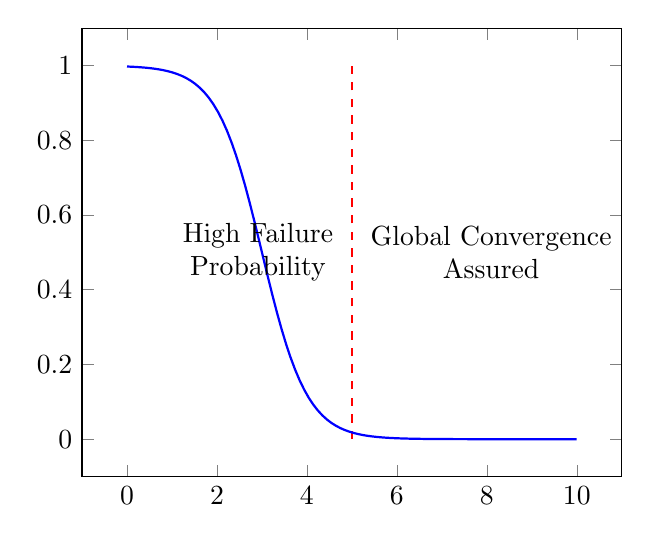
\begin{tikzpicture}
        \begin{axis}[
            % Optional: You can uncomment the line below to make the plot wider
            % width=12cm,
        ]
        
        % Vertical line for Pataki bound
        \addplot[dashed, red, thick] coordinates {(5,0) (5,1)};
        
        % Curve showing decreasing probability
        \addplot[blue, thick, domain=0:10, samples=100] {1 / (1 + exp(2*(x-3)))};
        
        % FIX: Added align=center and line breaks (\\) to fit the text inside the bounds
        % Changed anchors to 'west' and 'east' for better vertical centering
        \node[anchor=west, text=black, align=center] at (axis cs:5.2,0.5) {Global Convergence \\ Assured};
        \node[anchor=east, text=black, align=center] at (axis cs:4.8,0.5) {High Failure \\ Probability};
        
        \end{axis}
    \end{tikzpicture}
    \caption{Visualizing the transition of the non-convex landscape. As the inner rank $p$ exceeds the critical Barvinok-Pataki threshold, the likelihood of encountering spurious local minima collapses to zero, yielding a landscape populated solely by global optima and strict saddle points.}
    \label{fig:pataki_threshold}
\end{figure}

\vspace{12cm}

\begin{figure}[h!]
    \centering
    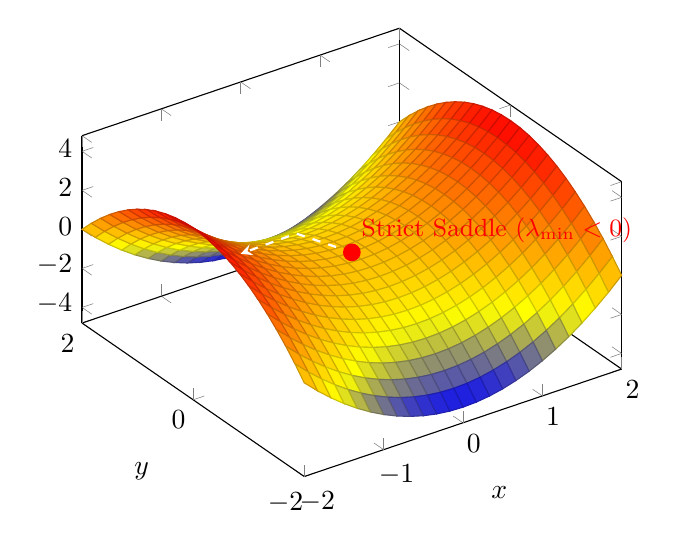
\begin{tikzpicture}
        \begin{axis}[
            clip=false,
            view={-35}{45},
            colormap/hot,
            xlabel=$x$, ylabel=$y$
        ]
        \addplot3[
            surf,
            domain=-2:2,
            domain y=-2:2,
            samples=25,
        ] {x^2 - y^2};
        
        % Plot the critical point (0,0,0)
        \addplot3[mark=*, mark size=3pt, color=red] coordinates {(0,0,0)};
        \node[red, anchor=south west] at (axis cs:0,0,0) {\small Strict Saddle ($\lambda_{\min} < 0$)};
        
        % Plot SGD escape trajectory
        \addplot3[thick, dashed, white, -stealth] coordinates {(0,0,0) (0,1,-1) (0,2,-4)};
        
        \end{axis}
    \end{tikzpicture}
    \caption{A 3D surface representation of a Strict Saddle Point on the quotient manifold. The topology illustrates a first-order critical point ($\nabla f = 0$), yet the presence of a strictly negative Hessian eigenvalue generates a distinct valley of descent. The dashed line illustrates how stochastic noise perturbs the trajectory off the plateau, allowing gradient descent to escape.}
    \label{fig:strict_saddle_topology}
\end{figure}